\documentclass[12pt,a4paper]{article}

% Paquetes esenciales para tipografía y formato académico
\usepackage[utf8]{inputenc}
\usepackage[T1]{fontenc}
\usepackage{lmodern} % Tipografía Latin Modern - alta legibilidad
\usepackage{microtype} % Mejoras tipográficas finas
\usepackage{geometry} % Control de márgenes
\usepackage{setspace} % Control de interlineado
\usepackage{graphicx} % Para imágenes
\usepackage{float} % Control de posición de figuras
\usepackage{caption} % Mejoras en captions
\usepackage{subcaption} % Subfiguras
\usepackage{booktabs} % Tablas profesionales
\usepackage{array} % Mejoras en tablas
\usepackage{multirow} % Celdas múltiples en tablas
\usepackage{tabularx} % Tablas con ancho ajustable
\usepackage{longtable} % Tablas multipágina
\usepackage{adjustbox} % Ajuste de cajas y tablas
\usepackage{xcolor} % Colores
\usepackage{hyperref} % Enlaces y PDF interactivo
\usepackage{fancyhdr} % Encabezados y pies de página
\usepackage{enumitem} % Listas mejoradas
\usepackage{titlesec} % Títulos personalizados

% Configuración de márgenes optimizada para formato académico
\geometry{
    a4paper,
    left=2.5cm,      % Margen izquierdo estándar académico
    right=2.5cm,     % Margen derecho
    top=2.5cm,       % Margen superior
    bottom=2.5cm,    % Margen inferior
    headheight=15pt,
    headsep=20pt,
    footskip=30pt
}

% Configuración de interlineado para mejor legibilidad
\renewcommand{\baselinestretch}{1.3} % 1.3 de interlineado (estándar académico)

% Configuración de colores para alto contraste
\definecolor{darkblue}{RGB}{0,51,102}
\definecolor{lightgray}{RGB}{245,245,245}

% Configuración de hyperref para accesibilidad
\hypersetup{
    colorlinks=true,
    linkcolor=darkblue,
    filecolor=darkblue,
    urlcolor=darkblue,
    citecolor=darkblue,
    bookmarks=true,
    bookmarksopen=true,
    bookmarksnumbered=true,
    pdfstartview=FitH
}

% Configuración de fuentes y tamaños
\setlength{\parindent}{0pt} % Sin sangría
\setlength{\parskip}{8pt} % Espacio entre párrafos

% Configuración de títulos estilo académico
\titleformat{\section}{\Large\bfseries\scshape}{\thesection}{1em}{}
\titleformat{\subsection}{\large\bfseries}{\thesubsection}{1em}{}
\titleformat{\subsubsection}{\normalsize\bfseries}{\thesubsubsection}{1em}{}

% Espaciado entre secciones
\titlespacing*{\section}{0pt}{20pt}{10pt}
\titlespacing*{\subsection}{0pt}{15pt}{8pt}
\titlespacing*{\subsubsection}{0pt}{12pt}{6pt}

% Configuración de encabezado y pie de página
\pagestyle{fancy}
\fancyhf{}
\fancyhead[L]{\small\textsc{EPRO Grupo 1}}
\fancyhead[R]{\small\textsc{Universidad Escuela Colombiana de Ingeniería}}
\fancyfoot[C]{\small\thepage}
\renewcommand{\headrulewidth}{0.4pt}
\renewcommand{\footrulewidth}{0pt}

% Comandos personalizados para consistencia
\newcommand{\sectiontitle}[1]{\section{#1}}
\newcommand{\subsectiontitle}[1]{\subsection{#1}}
\newcommand{\subsubsectiontitle}[1]{\subsubsection{#1}}
\newcommand{\tablecaption}[1]{\caption{#1}}

% Configuración para tablas
\renewcommand{\arraystretch}{1.2} % Espacio en celdas de tabla
\setlength{\tabcolsep}{8pt} % Espacio entre columnas

% Configuración para figuras
\captionsetup[figure]{font=small,labelfont=bf}
\captionsetup[table]{font=small,labelfont=bf}

% Configuración de listas
\setlist[itemize]{leftmargin=*,itemsep=5pt,topsep=5pt}
\setlist[enumerate]{leftmargin=*,itemsep=5pt,topsep=5pt}

% Comando para tablas anchas
\newcommand{\adjusttable}[1]{%
  \begin{adjustbox}{width=\textwidth,center}
    #1
  \end{adjustbox}
}

% Información del documento
\title{\textbf{MONTAJE DE UNA EMPRESA DE RESERVAS CON PLANIFICACIÓN DE VIAJE,}\\
A TRAVÉS DE UNA APLICACIÓN EN COLOMBIA}
\author{EPRO Grupo 1\\
    \small Santiago Botero García\\
    \small Juana Lozano Chaves\\
    \small Juan Pablo Salamanca Mojica\\
    \small Sofia Velandia Cifuentes\\
    \small Laura Alejandra Venegas Piraban\\
    \vspace{0.5cm}
    \small Profesor: Daniel Salazar Ferro}
\date{BOGOTÁ, COLOMBIA}

\begin{document}

% Página de título
\begin{titlepage}
    \centering
    \vspace*{2cm}
    
    {\Large\textbf{UNIVERSIDAD ESCUELA COLOMBIANA DE INGENIERÍA JULIO GARAVITO}}\\[1cm]
    
    {\Large\textbf{MONTAJE DE UNA EMPRESA DE RESERVAS CON PLANIFICACIÓN DE VIAJE,}}\\[0.3cm]
    {\Large A TRAVÉS DE UNA APLICACIÓN EN COLOMBIA}\\[2cm]
    
    {\large\textbf{EPRO GRUPO 1}}\\[1.5cm]
    
    \textbf{Estudiantes:}\\[0.5cm]
    JUAN PABLO SALAMANCA MOJICA\\
    JUANA LOZANO CHAVES\\
    LAURA ALEJANDRA VENEGAS\\
    SANTIAGO BOTERO GARCÍA\\
    SOFÍA VELANDIA CIFUENTES\\[1.5cm]
    
    \textbf{Profesor:}\\[0.5cm]
    Daniel Salazar Ferro\\[2cm]
    
    \textbf{BOGOTÁ, COLOMBIA}
    
    \vfill
\end{titlepage}

% Tabla de contenidos
\tableofcontents
\newpage

% Contenido principal
\sectiontitle{NOMBRE DEL PROYECTO}

\textbf{MONTAJE DE UNA EMPRESA DE RESERVAS CON PLANIFICACIÓN DE VIAJE A TRAVÉS DE UNA APLICACIÓN EN COLOMBIA}

\sectiontitle{PROPÓSITO DEL PROYECTO Y OBJETIVO ESTRATÉGICO DE LA ORGANIZACIÓN AL CUAL CONTRIBUYE}

\subsectiontitle{PROPÓSITO DEL PROYECTO:}

\begin{itemize}
    \item Superar las limitaciones de los sistemas de reserva turísticos actuales en Colombia.
    \item Aprovechar el crecimiento del turismo mediante una plataforma digital integrada.
    \item Facilitar la búsqueda, comparación y reserva de servicios turísticos en un solo sistema.
    \item Mejorar la toma de decisiones de los usuarios a través de información y reseñas confiables.
    \item Incrementar la visibilidad y competitividad de los proveedores turísticos.
\end{itemize}

\subsectiontitle{ALINEACIÓN ESTRATÉGICA:}

\begin{table}[H]
\centering
\begin{tabular}{p{3.5cm}p{4cm}p{5.5cm}}
\toprule
\textbf{Organización} & \textbf{Objetivos estratégicos} & \textbf{Aportes del Proyecto} \\
\midrule
\textbf{Ministerio de Comercio, Industria y Turismo (MinCIT)} & Incrementar la competitividad y sostenibilidad del turismo colombiano mediante transformación digital. & Plataforma integrada que mejora la planificación, reservas y visibilidad del sector turístico nacional. \\
\addlinespace
\textbf{FONTUR (Fondo Nacional de Turismo)} & Fortalecer la infraestructura turística y la digitalización del sector. & Herramienta tecnológica escalable que apoya proyectos de innovación, promoción y modernización turística. \\
\addlinespace
\textbf{Institutos y Secretarías de Turismo (IDT Bogotá, Secretarías Departamentales y Municipales)} & Promover destinos, redistribuir la demanda y mejorar la experiencia del visitante. & Canal digital que visibiliza la oferta local, descongestiona destinos saturados y mejora la gestión territorial del turismo. \\
\addlinespace
\textbf{ProColombia} & Posicionar a Colombia como destino turístico competitivo a nivel internacional. & Plataforma que mejora la experiencia del turista extranjero y fortalece la percepción de Colombia como destino digitalmente avanzado. \\
\addlinespace
\textbf{Prestadores de Servicios Turísticos (Hoteles, operadores, guías, transporte, cultura)} & Aumentar ventas directas, visibilidad y eficiencia operativa. & Reducción de intermediación, acceso a reservas digitales, analítica de demanda y herramientas de gestión comercial. \\
\bottomrule
\end{tabular}
\caption{Alineación estratégica del proyecto con organizaciones del sector turístico}
\end{table}

\sectiontitle{PROBLEMAS DEL PROYECTO}

\begin{figure}[H]
\centering
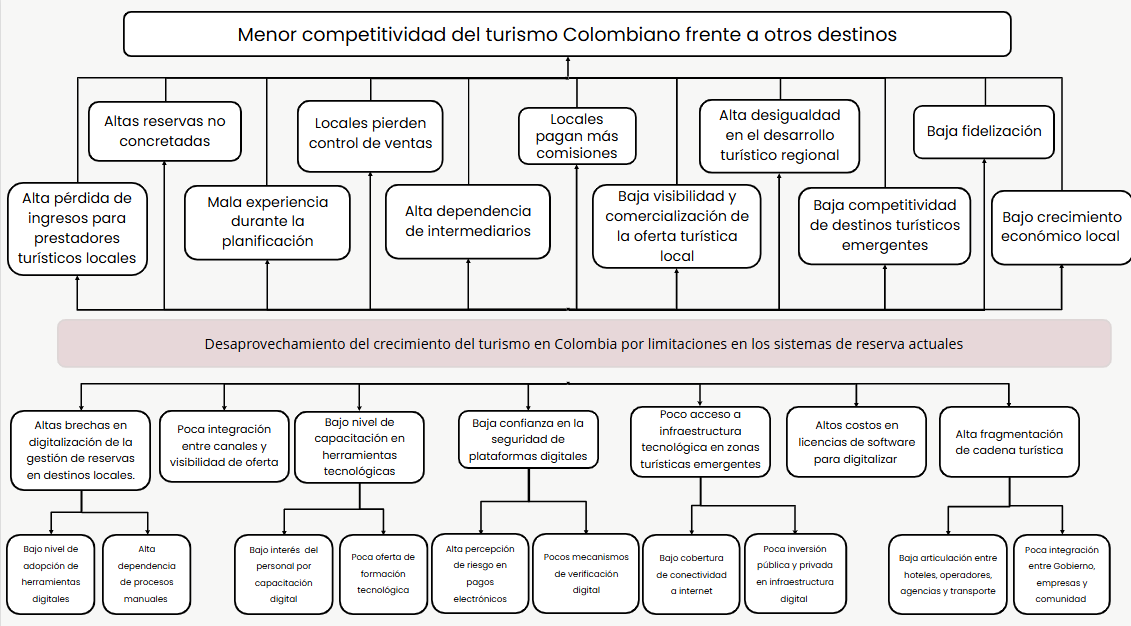
\includegraphics[width=0.8\textwidth]{img/Planteamiento_Proyecto_img-006.png}
\caption{Árbol de Problemas del proyecto}
\end{figure}

\sectiontitle{OBJETIVOS DEL PROYECTO}

\begin{figure}[H]
\centering
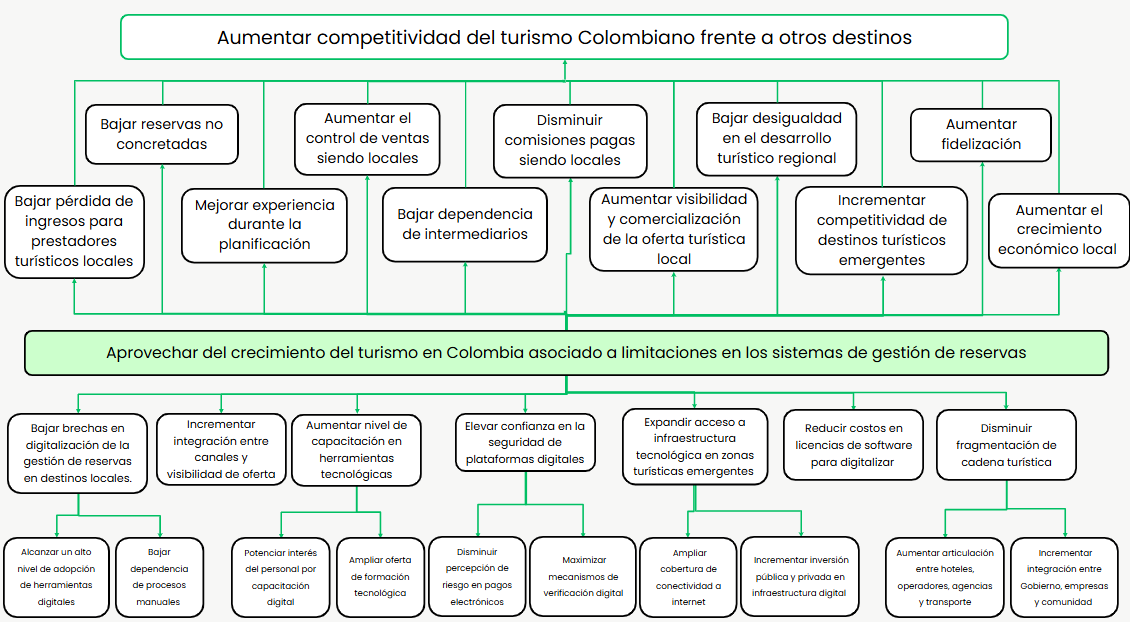
\includegraphics[width=0.8\textwidth]{img/Planteamiento_Proyecto_img-005.png}
\caption{Árbol de Objetivos del proyecto}
\end{figure}

\subsectiontitle{OBJETIVO GENERAL}

Desarrollar e implementar una plataforma digital integral de reservas y planificación de viajes que conecte a viajeros con proveedores turísticos en Colombia, mejorando la experiencia del usuario y fortaleciendo el sector turístico nacional.

\subsectiontitle{OBJETIVOS ESPECÍFICOS}

\begin{enumerate}
    \item \textbf{Desarrollar una plataforma tecnológica robusta:} Crear una aplicación móvil y web con funcionalidades de reservas, planificación algorítmica de viajes y red social de viajeros.
    \item \textbf{Integrar proveedores turísticos:} Conectar hoteles, transportes, guías y operadores turísticos de todo el territorio nacional.
    \item \textbf{Implementar sistemas de pago seguros:} Integrar pasarelas de pago confiables y certificadas para transacciones seguras.
    \item \textbf{Desarrollar algoritmos de recomendación:} Crear sistemas de IA que personalicen las recomendaciones de viajes según preferencias del usuario.
    \item \textbf{Establecer alianzas estratégicas:} Formar partnerships con entidades gubernamentales y privadas del sector turístico.
    \item \textbf{Garantizar accesibilidad y usabilidad:} Diseñar interfaces intuitivas y accesibles para diferentes perfiles de usuarios.
\end{enumerate}

\sectiontitle{ALCANCE DEL PROYECTO}

\subsectiontitle{ALCANCE INCLUIDO}

\begin{itemize}
    \item Desarrollo de aplicación móvil (iOS y Android) y plataforma web.
    \item Sistema de reservas en tiempo real para alojamientos, transportes y actividades.
    \item Algoritmos de planificación automática de itinerarios.
    \item Red social para viajeros con reseñas y recomendaciones.
    \item Sistema de pagos integrado con múltiples métodos de pago.
    \item Panel de control para proveedores turísticos.
    \item Sistema de calificación y reseñas verificadas.
    \item Integración con APIs de proveedores turísticos establecidos.
\end{itemize}

\subsectiontitle{ALCANCE EXCLUIDO}

\begin{itemize}
    \item Operación directa de servicios turísticos (hoteles, transportes, etc.).
    \item Gestión de visas y documentos de viaje internacionales.
    \item Seguros de viaje (solo integración con proveedores externos).
    \item Reservas de vuelos internacionales directos (solo integración).
    \item Servicios de cambio de divisas.
    \item Operación de call centers para atención al cliente (solo canales digitales).
\end{itemize}

\sectiontitle{STAKEHOLDERS DEL PROYECTO}

\subsectiontitle{STAKEHOLDERS PRIMARIOS}

\begin{itemize}
    \item \textbf{Viajeros y turistas:} Usuarios finales de la plataforma.
    \item \textbf{Proveedores turísticos:} Hoteles, restaurantes, transportes, guías, operadores.
    \item \textbf{Equipo del proyecto:} Desarrolladores, diseñadores, gerentes de proyecto.
    \item \textbf{Inversores:} Financiadores del proyecto.
\end{itemize}

\subsectiontitle{STAKEHOLDERS SECUNDARIOS}

\begin{itemize}
    \item \textbf{Entidades gubernamentales:} MinCIT, FONTUR, ProColombia, secretarías de turismo.
    \item \textbf{Asociaciones del sector:} ANATO, COTELCO, gremios turísticos.
    \item \textbf{Proveedores tecnológicos:} AWS, pasarelas de pago, proveedores de APIs.
    \item \textbf{Competidores:} Booking.com, Airbnb, Despegar, plataformas locales.
\end{itemize}

\sectiontitle{CRONOGRAMA DEL PROYECTO}

\begin{figure}[H]
\centering
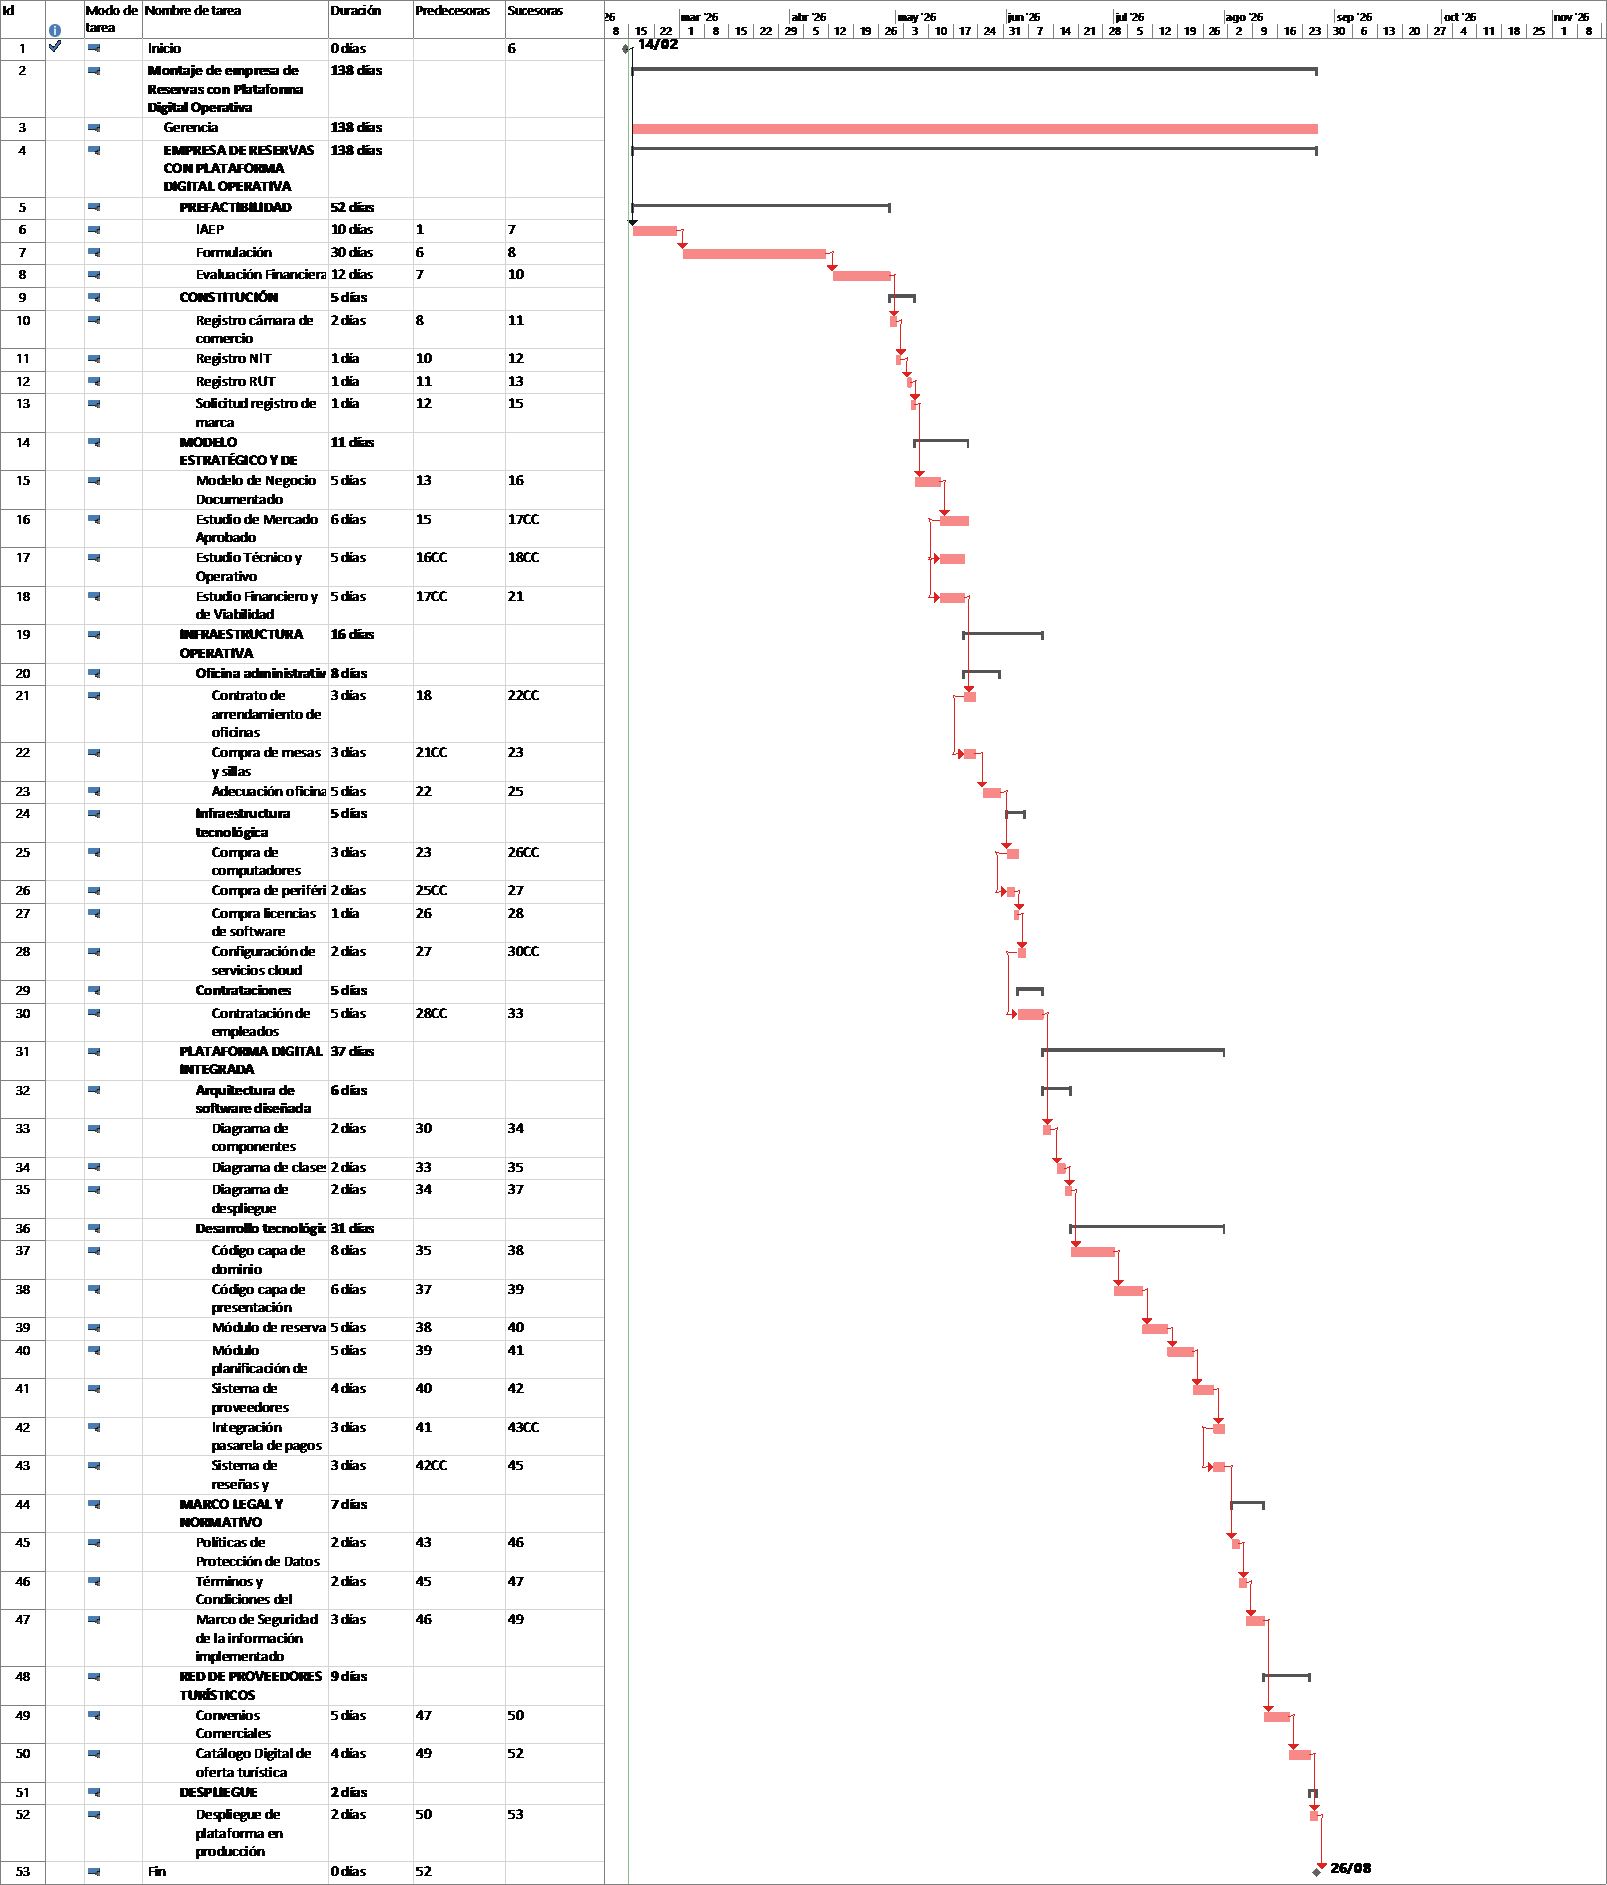
\includegraphics[width=0.9\textwidth]{img/Planteamiento_Proyecto_img-007.png}
\caption{Cronograma del proyecto en MS Project}
\end{figure}

\subsectiontitle{FASE 1: PLANEACIÓN Y DISEÑO (MESES 1-3)}

\begin{itemize}
    \item Investigación de mercado y análisis de competencia.
    \item Diseño de arquitectura tecnológica.
    \item Diseño de experiencia de usuario (UX) e interfaz (UI).
    \item Definición de requisitos funcionales y no funcionales.
    \item Selección de stack tecnológico y proveedores.
\end{itemize}

\subsectiontitle{FASE 2: DESARROLLO MÍNIMO VIABLE (MESES 4-9)}

\begin{itemize}
    \item Desarrollo del backend y base de datos.
    \item Desarrollo de APIs principales.
    \item Desarrollo de aplicación móvil básica.
    \item Integración con pasarelas de pago.
    \item Integración con proveedores turísticos iniciales.
\end{itemize}

\subsectiontitle{FASE 3: PRUEBAS Y LANZAMIENTO (MESES 10-12)}

\begin{itemize}
    \item Pruebas de usabilidad y rendimiento.
    \item Programa piloto con usuarios seleccionados.
    \item Ajustes y optimización del sistema.
    \item Lanzamiento oficial al mercado.
    \item Campañas de marketing inicial.
\end{itemize}

\subsectiontitle{FASE 4: ESCALAMIENTO Y EXPANSIÓN (MESES 13-18)}

\begin{itemize}
    \item Incorporación de nuevas funcionalidades.
    \item Expansión a nuevos segmentos de mercado.
    \item Optimización de algoritmos de recomendación.
    \item Expansión de red de proveedores.
    \item Internacionalización gradual.
\end{itemize}

\sectiontitle{PRESUPUESTO ESTIMADO}

\begin{figure}[H]
\centering
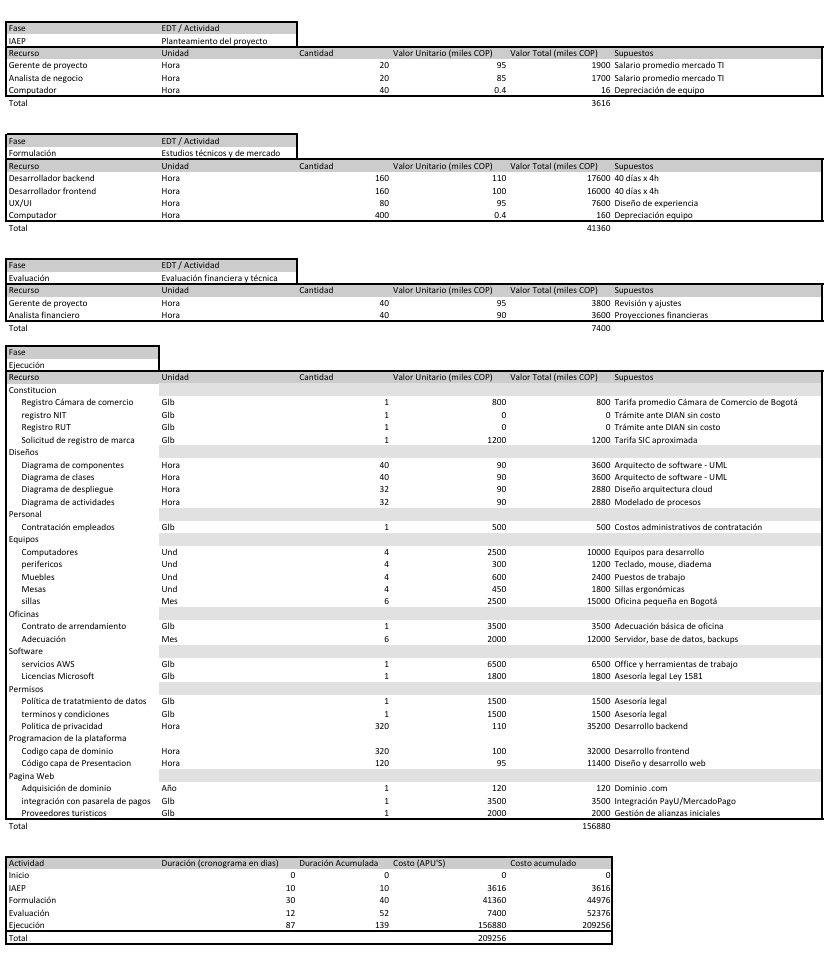
\includegraphics[width=0.9\textwidth]{img/Planteamiento_Proyecto_img-009.png}
\caption{Presupuesto estimado del proyecto}
\end{figure}

\subsectiontitle{INVERSIÓN INICIAL}

\begin{itemize}
    \item \textbf{Desarrollo tecnológico:} \$150.000.000 COP
    \item \textbf{Infraestructura y licencias:} \$45.000.000 COP/año
    \item \textbf{Marketing y lanzamiento:} \$80.000.000 COP
    \item \textbf{Operaciones iniciales:} \$60.000.000 COP/año
    \item \textbf{Legal y constitución:} \$25.000.000 COP
\end{itemize}

\subsectiontitle{COSTOS OPERATIVOS ANUALES}

\begin{itemize}
    \item \textbf{Mantenimiento tecnológico:} \$90.000.000 COP
    \item \textbf{Servicios cloud:} \$54.000.000 COP
    \item \textbf{Personal operativo:} \$180.000.000 COP
    \item \textbf{Marketing continuo:} \$120.000.000 COP
    \item \textbf{Servicios profesionales:} \$36.000.000 COP
\end{itemize}

\sectiontitle{INDICADORES DE ÉXITO (KPIs)}

\subsectiontitle{KPIs DE ADOPCIÓN}

\begin{itemize}
    \item Número de usuarios registrados: 10.000 en el primer año.
    \item Tasa de conversión de reservas: 15\% de usuarios activos.
    \item Retención de usuarios: 60\% después de 6 meses.
    \item Número de proveedores activos: 500 en el primer año.
\end{itemize}

\subsectiontitle{KPIs FINANCIEROS}

\begin{itemize}
    \item Volumen de transacciones: \$2.000.000.000 COP en el primer año.
    \item Ingresos por comisiones: \$200.000.000 COP en el primer año.
    \item Costo de adquisición de cliente (CAC): \$15.000 COP por usuario.
    \item Valor de vida del cliente (LTV): \$150.000 COP por usuario.
\end{itemize}

\subsectiontitle{KPIs DE SATISFACCIÓN}

\begin{itemize}
    \item Calificación promedio de la aplicación: 4.2/5 estrellas.
    \item Tasa de satisfacción del cliente (CSAT): 85\%.
    \item Número neto de promotores (NPS): 45.
    \item Tiempo de respuesta de soporte: < 2 horas.
\end{itemize}

\end{document}
